In order to improve the performance of the svm model I tried modifying the scheduler
and the optimizer. I noticed that using SDG with a StepLR scheduler I was able to 
surpass the accuracies of KNN and Nearest Centroid even though I was still behind MLP.
MLP has one hidden layer making it able to deal with more complex problems and thus 
it is expected to outperform the other algorithms. Here are the results of the SVM 
model with the modifications:
\begin{figure}[H]
    \centering
    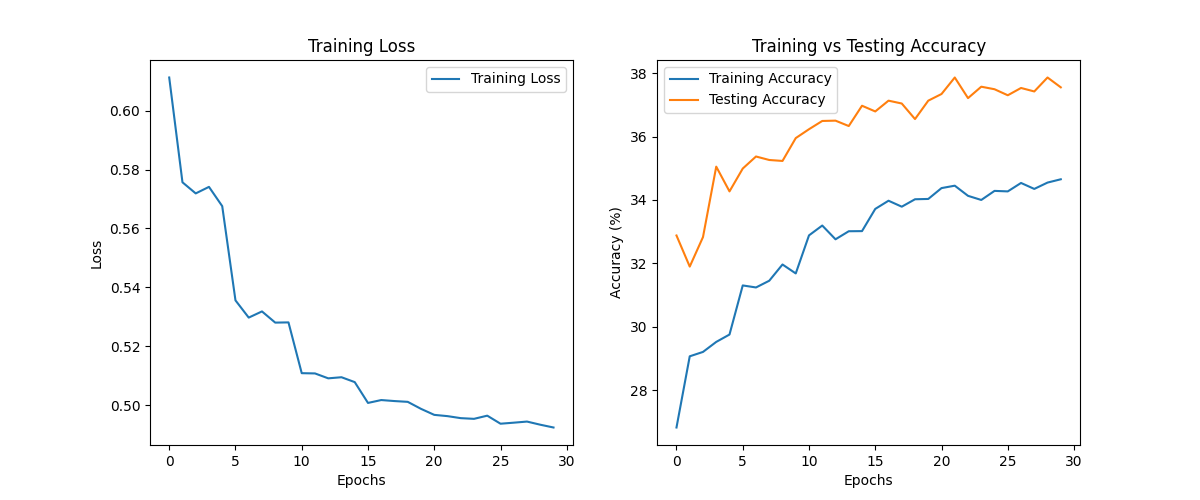
\includegraphics[width=0.5\textwidth]{media/svm_modified.png}
    \caption{SVM with SDG and StepLR scheduler}
\end{figure}
Training Completed in 5.35 minutes \\
Best Test Accuracy: 37.86\% \\

\smallskip

Let's break down why the performance improved, but first some general information
about the two SVM variations.
\begin{itemize}
    \item Adam optimizer with ReduceLROnPlateau scheduler
    \begin{itemize}
        \item Adam learning rate: 0.01
        \item ReduceLROnPlateau patience: 3
        \item ReduceLROnPlateau factor: 0.5
    \end{itemize}
    \item SGD optimizer with StepLR scheduler
    \begin{itemize}
        \item SGD learning rate: 0.01
        \item SGD weight decay: 0.0005
        \item SGD momentum: 0.9
        \item StepLR step size: 5
        \item StepLR gamma: 0.5
    \end{itemize}
\end{itemize}
Learning rates are kept the same for both optimizers to make the comparison fair.
They specify the step size at each iteration while moving toward a minimum of the 
loss function. The main difference between the two optimizers is that Adam is an 
adaptive learning rate optimization algorithm while SGD is a stochastic gradient 
descent algorithm. SGD has two additional parameters when compared to Adam:
\begin{itemize}
    \item Weight decay: Regularization term that penalizes large weights.
    \item Momentum: Accelerates the gradient descent by adding a fraction of the
    previous weight update to the current update. 
\end{itemize}

Reduce on Plateau is a scheduler that reduces the learning rate when a metric has 
stopped improving. In our case that metric is test\_loss. The scheduler has two 
important parameters:
\begin{itemize}
    \item Patience: Determines how many epochs to wait before reducing the learning 
    rate. 
    \item Factor: Determines how much to reduce the learning rate by.
\end{itemize}
On the other hand the StepLR scheduler reduces the learning rate by a factor every
fixed number of epochs. The scheduler has two important parameters:
\begin{itemize}
    \item Step size: Determines how many epochs to wait before reducing the learning 
    rate.
    \item Gamma: Determines how much to reduce the learning rate by.
\end{itemize}

Thus we can conclude based on our observations and the information above that the
SVM model is favored by a fixed scheduler and a stochastic gradient descent optimizer.
It has to be noted that reducing patience and factor on the Adam/ReduceLROnPlateau 
model did make the model learn faster and achieve slightly better accuracy in the end 
but it still lost to the StepLR scheduler. However, it isn't just the scheduler since 
Adam with the StepLR scheduler was once again 2\% behind the SDG/StepLR model. The 
fixed and steep learning rate reduction along with the momentum and weight decay
of the SGD marked a slight improvement in the performance of the SVM model, enough
to surpass KNN and Nearest Centroid.
